\documentclass[12pt]{article}

\usepackage[margin=1.25in]{geometry}
\usepackage[english]{babel}
\usepackage[utf8]{inputenc}
\usepackage{amsmath}
\usepackage{graphicx}
\usepackage[colorinlistoftodos]{todonotes}
\usepackage{cite}
\usepackage{tikz}



\title{Real-time Sentiment Analysis of Twitch Chats}

\author{William Klock}

\date{\today}

\begin{document}
\maketitle

\begin{abstract}
An attempt to obtain meaningful sentiment from chats associated with live-stream events on Twitch.com. The project uses a pair of Naïve-Bayes classifiers trained on the Sentiment140 and movie-review data from NLTK run in parallel to determine if there is a solid subtext to the chat messages. The results are inconclusive.
\end{abstract}

\section{Introduction}

Sentiment analysis has been a widely researched topic within computational linguistics in the recent years. The goal: find more ways to train a computer to gather information about the attitude of a text. This information is important because a lot of information is lost during computation because computers do not have an innate understanding of a piece of writing's subtext. Additionally, one of the main distinctions between human and computer language is emotion. Although teaching a computer to understand sentiment is still far off from making a computer that is emotionally intelligent, it is an important step in making computers more aware overall.

Instead of trying to improve current techniques, this project attempts to analyze a new source of data: chat streams associated with live-video broadcasting. The motivation being that understanding the current sentiment of a broadcast will give insights that could aid in wagering against the outcome, potentially for monetary gain. This paper focuses on Twitch.com, a platform for streaming video games. Although this area is niche, its popularity is on the rise, and thus the motivation for seeking understanding is higher than ever. 

\section{Problem Definition}
The first question is whether or not it is possible to retrieve valuable information from a live stream chat using readily available linguistic processing methods. Although the answer may seem trivial, looking at the excerpt in Figure 1, it becomes obvious that whether or not the messages are meaningful is unclear.

The second question is whether or not the potential information can be extracted in real time. Typically linguistic processing is something that is done without regard to running-time, but in this situation, maintaining an up-to-date sentiment score is critical because the information is relevant for only a moment within the context of the stream. Usually in these streams there are many participants, which means many messages are sent each second, which requires a non-standard approach to generate accurate data.

\begin{figure}
\centering
	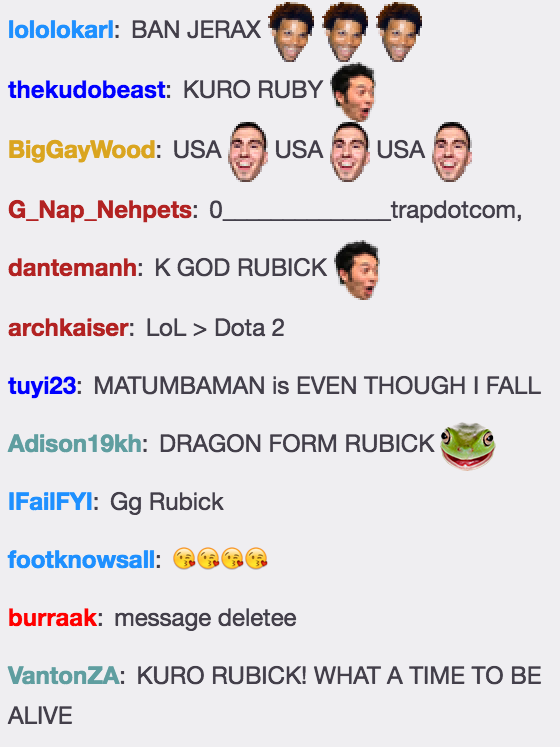
\includegraphics[height=3in]{example.png}
	\caption{\label{fig:chat}An excerpt from a chat on Twitch during a DOTA2 live-steam with over 80,000 viewers}
\end{figure}

\section{Previous Work}
Throughout the last decade there has been an incredible amount of work done in the field of sentiment analysis. A comprehensive look on sentiment analysis is given in \cite{Liu2012}, so the focus of this section will be on research related to this topic.

Despite much work has been done on sentiment analysis, no previous work has attempted an analysis of texts as short or as informal as the chat-streams on \textit{Twitch}. Throughout the literature, the shortest and most informal data used are tweets. Even though Twitter imposes a 140 character limit on each tweet this is much longer than the majority of the messages sent on Twitch. Additionally, because the relevance of a tweet is much longer than the period of relevance for a message in a chat, tweets tend to be more formal than any particular message in a chat. 

Disregarding the inherent differences in the problem, the most similar article, \cite{Kiritchenko:1} uses state-of-the-art techniques to gather sentiment from tweets and SMS messages. The team achieved an F-score of 70.45 on Semeval-2013 tweet data and an F-score of 69.77 on SMS data. Since SMS messages are similar to the messages tested on in this paper, there is hope for valuable information extraction from Twitch messages.

Given appropriate assurance that a computer can extract information from texts similar to the Twitch messages that are the focus here, the next step is determining an appropriate approach. The work by Go, Bhayani, and Huang \cite{go2009twitter} show that a Naïve-Bayes classifier performs well on Twitter sentiment analysis. Given that Naïve-Bayes does not require intense computation compared to the alternatives (support vector and maximum entropy). 
 

\section{Approach}

There were two constraints when considering the approach to solve this problem: time and computational power. The time constraint limits the scope of the project and the amount of data that can be gathered. Since the work was done on a 2013 MacBook Pro, the compute power limits the size of the data set and the types of classifiers that can be used. 

Given the task of determining whether or not Twitch messages contain detectable sentiment, two classifiers will be trained on different sets of training data and the output from the two classifiers will be compared. If the classifiers agree with each other the majority of the time, the information from either of them will be deemed useful, and the sentiment of the message deemed valid. 

The first step is to gather the messages from Twitch. Twitch uses the Internet Relay Chat Protocol (IRCP) as the framework that underlies the web based chat, shown in Figure 1. A connection can be established programmatically, in this case with Python, and the server will relay the messages to the client in the form:
\begin{quote}
\begin{center}
\begin{verbatim}
	:kaysome_vg!kaysome_vg@kaysome_vg.tmi.twitch.tv
	 PRIVMSG #bacon_donut :Haha, he's here
\end{verbatim}
\end{center}
\end{quote}

Here, the only valuable piece of the message is, "Haha, he's here," which can be singled out through basic string manipulation. 

With the chat data in hand, the second step is to decide what training data to use. The two data sets chosen were a subset of the Sentiment140 Lexicon used in \cite{go2009twitter} and \cite{MohammadKZ2013} and the NLTK Twitter data set, available through the command-line. Since the Sentiment140 set contains around 1.6 million entries, I could only use a subset of the data because of the limited computational resources available. These two datasets were chosen mostly for their prevalence in the literature and the ease with which they could be obtained.

The next step is determining an appropriate classifier for the problem. With the constraints in mind, a binary Naïve-Bayes classifier (NBC) is the simplest solution because of its ease-of-use and effectiveness relative to computation time required during training. Previous work has shown that a well-trained NBC performs near the cutting edge of current research. For this research, two Naïve-Bayes classifiers were trained: one on the Sentiment140 data, and one on the NLTK data.

Finally, each of these components are brought together in a parallelized system that spawns a new thread for each message and prints out its sentiment. The layout is given below. 
\begin{center}
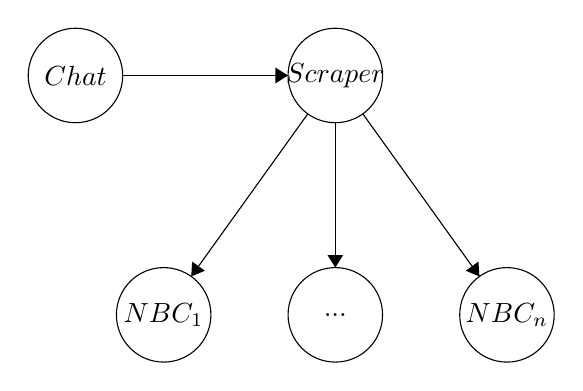
\begin{tikzpicture}[scale=0.2]
\tikzstyle{every node}+=[inner sep=0pt]
\draw [black] (13.6,-20.1) circle (3);
\draw (13.6,-20.1) node {$Chat$};
\draw [black] (30.1,-20.1) circle (3);
\draw (30.1,-20.1) node {$Scraper$};
\draw [black] (19.2,-35.3) circle (3);
\draw (19.2,-35.3) node {$NBC_1$};
\draw [black] (30.1,-35.3) circle (3);
\draw (30.1,-35.3) node {$...$};
\draw [black] (41,-35.3) circle (3);
\draw (41,-35.3) node {$NBC_n$};
\draw [black] (16.6,-20.1) -- (27.1,-20.1);
\fill [black] (27.1,-20.1) -- (26.3,-19.6) -- (26.3,-20.6);
\draw [black] (28.35,-22.54) -- (20.95,-32.86);
\fill [black] (20.95,-32.86) -- (21.82,-32.5) -- (21.01,-31.92);
\draw [black] (30.1,-23.1) -- (30.1,-32.3);
\fill [black] (30.1,-32.3) -- (30.6,-31.5) -- (29.6,-31.5);
\draw [black] (31.85,-22.54) -- (39.25,-32.86);
\fill [black] (39.25,-32.86) -- (39.19,-31.92) -- (38.38,-32.5);
\end{tikzpicture}
\end{center}

\section{Results}
To determine whether or not there is valid information within Twitch messages, the outputs of the two classifiers were compared and if the majority ($>50\%$) of the output was in agreement, then the message was said to have enough information. Looking at the outputs of multiple streams, the classifiers agreed about half the time, but there is a caveat. The classifier trained on the Sentiment140 data labelled every message as positive, which means that it is unlikely that the classifier was accurate on this data set. Therefore, it is impossible to draw a sound conclusion because the intermediate data required appears to be faulty.

As for the second part of the project, to obtain real-time analysis of the chat, the parallel approach used here was able to successfully process the messages as they were delivered. In fact, the system could have processed many streams at once because of the efficiency gained in doing the analysis in parallel.

\section{Discussion}
\subsection{Technical Analysis}
Unfortunately, this project met its demise due to a major shortfall of one of the classifiers that was essential to analysis of the data. Looking from the bottom up, there are some possible fault points worth discussion.

First, although the movie review data provided varying sentiments for the messages, the Sentiment140 data seemed to provide no insights. This means two things. The first is that the movie review data may have created a classifier that gave out random results that happened to be varied but were as worthless as the constant output that the Sentiment140 classifier gave. The second is that because the Sentiment140 classifier had to be trained on a smaller subset of the entire lexicon, it missed important data that would have resulted in more accurate labelings of the messages in the chat.

Second, since neither dataset included emoticons as part of the data, a large portion of the dataset was meaningless to the classifiers. Furthermore, instead of being innocuous, the emoticons could have altered the output of the classifier because they were not stripped from the input.

Either or a combination of these scenarios could have caused the failure of the classifier, but as this is research in computational linguistics and not machine learning, they are not the focus of the discussion.

\subsection{Theoretical Analysis}
From the non-technical the question must be asked of whether or not the inconclusive results indicate a lack of information within the messages, rather than a failure in machine training and classification. This notion must be entertained as it is entirely possible.  

If we consider the definition of sentiment, we find that it is a grandiose synonym for "opinion." Therefore, sentiment analysis is the analysis of opinion, and this definition could be the basis for a fundamental fault in this project. Perhaps it is the case that the messages sent in a Twitch chat are without opinion and instead represent a desire for lighthearted communication and inclusion. It could be the case, then that this project attempted to look too deep into a situation where there simply is no subtext worth analysis.

\subsection{Moving Forward}
There are many ways in which this experiment could be improved, a couple of which are discussed here:

The first is a manually labeled set of chat logs where each message had a sentiment assigned to it. This would potentially allow the classifiers to match the niche language of this sub-culture. The frequent use of emoticons and special vocabulary within the chats would likely have seen a great information gain from training data tailored to the scenario.

Another improvement to this study would have been to compare different varieties of classifiers such as maximum entropy and support vectors. Even if the training data were the same between them, the different methods could perhaps give better insights than a Naïve-Bayes classifier.
\pagebreak
\section{Conclusion}
Although this project failed in its attempt to find meaning in incredibly short and informal chat messages, it brought to light the question of whether or not all text has a deeper, underlying message, and even if it does, is it worth looking into. As society becomes more computationally based, it is important that language processing and synthetic intelligence as a whole keeps progressing in the right direction. Even though esoteric analyses of obscure data is interesting, perhaps now it is best to reconsider the questions we are asking of the world and its inhabitants, and ensure that the research done is done in a way that actively moves humanity forward.

\newpage
\bibliographystyle{plain}

\bibliography{mybib}{}
\end{document}
              
